% !TeX root = main.tex

\section{实现细节}
\label{sec:supp_settings}

\subsection{数据与词库}

表~\ref{tab:test_population} 汇总两个数据集的词库规模、候选数、训练词库覆盖率和测试范围。
训练词库只包含训练材料中的词。
验证选模时，从 $50$ 词候选中移除验证集未出现的词；测试时保留全部 $50$ 个候选。
ChineseEEG-2 依据实际朗读标点形成片段：在强标点处结束，弱标点后达到 $16$ 词时优先切分，
并将片段限制为最多 $32$ 词或 $15\,\mathrm{s}$，记录末尾保留剩余词位。

\begin{table}[htbp]
    \centering
    \papertablestyle
    \caption{词库、候选数及测试评价范围。查询数、片段数和词位数按一次模型评价计。}
    \label{tab:test_population}
    % Presentation only: simplify_appendix_tables_test_v2.py; verified frozen sources.
\begingroup
\papertablestyle
\begin{tabular}{@{}lrr@{}}
\toprule
项目 & Pallier2025 & ChineseEEG-2 \\
\midrule
训练词库 & 2020 & 2180 \\
训练词库覆盖率 & 82.49\% & 84.53\% \\
验证选模候选：词模型 & 50 & 47 \\
验证选模候选：上下文模型 & 49 & 46 \\
测试词检索候选 & 50 & 50 \\
\addlinespace
局部范围测试查询 & 8930 & 3444 \\
可见状态共同查询 & 7440 & 2872 \\
序列测试片段 & 1940 & 808 \\
序列参考词位 & 18450 & 8480 \\
序列材料块 & 39 & 21 \\
\bottomrule
\end{tabular}
\endgroup

\end{table}

文本表示由冻结的 BGE-M3 编码器得到。
每个词单独编码，取末层首个 token 的隐藏状态并做 $L_2$ 归一化：
\[
\mathbf y_i=\mathbf h_{i,\mathrm{first}}^{(L)}\big/\|\mathbf h_{i,\mathrm{first}}^{(L)}\|_2 .
\]


\subsection{模型与训练}
\label{sec:supp_model_training}

神经信号重采样至 $50$~Hz，主实验的 $1\,\mathrm{s}$ 词窗包含 $50$ 个时间点。
长窗对照分别使用 $64$ 和 $75$ 个时间点，对应 $1.28$ 和 $1.50\,\mathrm{s}$；
长窗词模型从头训练，沿用原词模型的训练配置和验证选模规则。
上下文 Transformer 为 $16$ 层、$16$ 个注意力头，隐藏维度 $1024$，
注意力 dropout 为 $0.1$，前馈层不使用 dropout。

词模型从头训练。
上下文模型加载同种子词模型的最佳检查点，新建上下文网络；
第一轮冻结神经编码器，之后联合训练。
两个阶段均使用 SigLIP 对比损失\cite{zhai2023siglip} 和 AdamW 优化器，
学习率 $10^{-4}$，余弦退火，批次大小 $128$，权重衰减 $0$，FP16 混合精度。
每阶段最多 $30$ 轮，验证指标连续 $10$ 轮未改善即停止。
检查点按验证集宏平均 Top-$10$ 选择：
词模型使用全部合格查询，上下文模型使用共同词位，共享滚动模型按 K2 选模。
各条件的输入和监督范围见表~\ref{tab:model_settings}。

\begin{table}[htbp]
    \centering
    \papertablestyle
    \caption{各模型的输入与训练设置。范围相对于目标词给出。独立 K2 与局部半径 $2$ 的输入和监督相同，使用同一个检查点。}
    \label{tab:model_settings}
    % Presentation only: simplify_appendix_tables_test_v2.py; verified frozen sources.
\begingroup
\papertablestyle
\begin{tabular}{@{}llll@{}}
\toprule
模型 & 输入范围 & 训练目标 & 参数关系 \\
\midrule
词模型 & 目标词神经窗 & 单词映射 & 不含上下文网络 \\
局部窗口 & $[-k,k]$ & 各词每轮一次 & 各半径分别训练 \\
完整上下文 & 片段内全部词 & 各词每轮一次 & 单独训练 \\
独立可见状态 & $[-2,r]$ & 各词每轮一次 & 各状态分别训练 \\
共享滚动模型 & $[-2,r]$ & \shortstack[l]{遍历到达时刻\\监督 K0/K1/K2} & 三个状态共享参数 \\
\bottomrule
\end{tabular}
\endgroup

\end{table}


\subsection{文本序列解码}
\label{sec:supp_sentence_settings}

语言模型对每个前缀生成若干条续写，每条只取第一个完整词作为候选，并去除重复。
两个数据集均使用连续叙述提示，提示中不包含刺激书名或内容：
法语为“Écrivez un paragraphe de récit en français. Donnez seulement le texte, sans titre ni liste.”；
中文为“请用中文写一段连续的叙述文字。只给出正文，不要标题或列表。”
提示后接两个换行，再拼接已解码前缀。

法语通常以空格连接词，但省音前项（如 c、j、l、d、qu）与后词之间插入撇号，
例如将 c 和 est 还原为 \textit{c'est}；以连字符开头的词直接接到前词。
中文词序列直接拼接，不插入空格。
前缀和加入候选后的文本分别整串编码，语言分数为两条整串文本的对数概率之差；
若拼接改变了边界 token，旧、新文本均从共同 token 前缀后的部分计算。
这避免将独立词编码的 token 概率直接拼接。
神经相似度乘以固定系数后，在训练词库和本步新提出的词库外候选上做 softmax。

语言权重使用验证材料上的种子 $0$、策略 A 的 WER 选择，平局时取较小值。
法语和中文分别选得 $\lambda=0.1$ 与 $0.5$，
同一数据集的全部策略和训练种子沿用相同提示、权重和搜索配置。
所有文本结果均按上述配置重新解码。

\begin{table}[!htbp]
    \centering
    \papertablestyle
    \caption{文本序列解码参数。两个数据集的语言权重分别选择；其余参数相同。}
    \label{tab:sentence_decoder_settings}
    % Rendered only from verified manuscript_text_stage3_v1 exports.
% Presentation only: verified reports/exports; polish_main_assets_test_v2.py.
\begingroup
\papertablestyle
\begin{tabular}{@{}lll@{}}
\toprule
设置 & Pallier2025 & ChineseEEG-2 \\
\midrule
语言模型 & \multicolumn{2}{l}{Qwen2.5-1.5B 基础版} \\
神经检索候选／词位 & \multicolumn{2}{l}{20} \\
神经相似度缩放系数 & \multicolumn{2}{l}{10} \\
束搜索保留序列数 & \multicolumn{2}{l}{5} \\
每个前缀的候选续写数 & \multicolumn{2}{l}{5} \\
每条续写的最大新 token 数 & \multicolumn{2}{l}{16} \\
近期重搜词位数（B/C） & \multicolumn{2}{l}{3} \\
语言模型上下文上限 & \multicolumn{2}{l}{32768 token} \\
验证语言权重候选 & \multicolumn{2}{l}{0, 0.025, 0.1, 0.5, 1.5} \\
语言权重选模指标 & \multicolumn{2}{l}{验证材料策略 A 的 WER} \\
权重平局规则 & \multicolumn{2}{l}{取较小值} \\
\midrule
测试固定语言权重 & 0.1 & 0.5 \\
\bottomrule
\end{tabular}
\endgroup

\end{table}

平均片段 BLEU-1 先在每个片段计算，再依次在受试者内、受试者间和种子间平均。
WER 和词位准确率按词位汇总，再对训练种子平均。

\subsection{统计方法}
\label{sec:statistics}
\label{sec:supp_statistics}

同一刺激在不同受试者中的呈现归为同一材料单元，每 $5$ 个连续材料单元构成一块，
在记录或章节内分层有放回抽样 $10000$ 次，取百分位数构造 $95\%$ 材料块 bootstrap 区间。
每次抽样对所有受试者、训练种子和比较条件使用相同的材料块，训练种子不另行重采样。
显著性检验采用双侧配对材料块符号翻转，使用 $1000000$ 次 Monte Carlo 抽样，
并按研究问题分组进行 Holm 多重比较校正；中文的 $21$ 个块另以全部 $2097152$ 种符号组合复核。
区间为点态区间，Holm 校正用于检验，不改变区间构造。
图中误差棒为三个训练种子的样本标准差。

\noindent\begin{minipage}{\linewidth}
ChineseEEG-2 中，
C$-$A 的 WER 差值为 $-1.57$ $[-2.07,-1.00]$ 个百分点，校正 $p=7.26\times10^{-4}$；词位准确率差值为 $+1.67$ $[1.07,2.19]$ 个百分点，校正 $p=7.26\times10^{-4}$。
C$-$B 的 WER 差值为 $-2.00$ $[-2.50,-1.48]$ 个百分点，校正 $p=4.80\times10^{-5}$；词位准确率差值为 $+2.08$ $[1.54,2.59]$ 个百分点，校正 $p=2.70\times10^{-5}$。
C$-$A 在两个数据集的三项文本指标组成的 $6$ 项比较内校正，
C$-$B 与 B$-$A 在两个数据集的三项指标组成的 $12$ 项比较内校正。
\end{minipage}

\clearpage
\section{完整词检索结果}
\label{sec:supp_word_statistics}

表~\ref{tab:word_complete_results} 给出 $50$ 词候选下全部模型的四项指标。
“全部”指真实词属于候选集合的全部合格查询，
“共同”进一步要求目标之后至少还有两个同片段词。
宏平均只在查询中实际出现的真实词类型上计算；
bootstrap 时按每次抽样实际出现的类型计算，两个比较条件使用相同的类型集合。

% Presentation only: formal test exports; consolidate_results_tables_test_v2.py.
\begingroup
\papertablestyle
\begin{longtable}{@{}lllrrrr@{}}
\caption{两个数据集的完整 $50$ 词候选检索结果（\%，三个种子均值 $\pm$ 样本标准差）。全部与共同查询分别列出；独立 K2 与局部半径 $2$ 共享检查点，比较时使用其共同查询行。}
\label{tab:word_complete_results}\label{tab:word_complete_pallier}\label{tab:word_complete_chinese}\\
\toprule
数据集 & 输入/模型 & 查询 & \shortstack{宏平均\\Top-$10$} & \shortstack{宏平均\\Top-$1$} & \shortstack{微平均\\Top-$10$} & \shortstack{微平均\\Top-$1$} \\
\midrule
\endfirsthead
\multicolumn{7}{l}{表~\ref{tab:word_complete_results}（续）}\\
\toprule
数据集 & 输入/模型 & 查询 & \shortstack{宏平均\\Top-$10$} & \shortstack{宏平均\\Top-$1$} & \shortstack{微平均\\Top-$10$} & \shortstack{微平均\\Top-$1$} \\
\midrule
\endhead
\midrule\multicolumn{7}{r}{续下页}\\\endfoot
\bottomrule\endlastfoot
Pallier2025 & 完整上下文 & 全部 & $65.52\pm0.31$ & $20.44\pm0.52$ & $68.53\pm0.78$ & $25.19\pm0.99$ \\
 &  & 共同 & $67.42\pm0.14$ & $21.23\pm0.47$ & $68.17\pm0.72$ & $24.66\pm1.04$ \\
\addlinespace
Pallier2025 & 局部半径 0 & 全部 & $38.16\pm1.15$ & $6.18\pm0.36$ & $36.91\pm0.97$ & $7.64\pm0.11$ \\
 &  & 共同 & $38.44\pm0.92$ & $6.15\pm0.24$ & $36.43\pm0.86$ & $7.22\pm0.06$ \\
\addlinespace
Pallier2025 & 局部半径 1 & 全部 & $67.00\pm1.50$ & $17.55\pm0.16$ & $67.18\pm1.47$ & $20.33\pm0.23$ \\
 &  & 共同 & $68.02\pm1.57$ & $17.59\pm0.25$ & $66.63\pm1.31$ & $19.26\pm0.22$ \\
\addlinespace
Pallier2025 & 局部半径 2 & 全部 & $70.62\pm0.34$ & $23.27\pm0.54$ & $72.95\pm0.23$ & $26.01\pm0.18$ \\
 &  & 共同 & $72.49\pm0.59$ & $23.55\pm0.55$ & $72.57\pm0.61$ & $24.86\pm0.37$ \\
\addlinespace
Pallier2025 & 局部半径 4 & 全部 & $68.38\pm0.63$ & $22.55\pm0.61$ & $71.02\pm1.33$ & $25.76\pm1.05$ \\
 &  & 共同 & $70.24\pm0.75$ & $23.17\pm0.91$ & $70.77\pm1.29$ & $25.09\pm0.80$ \\
\addlinespace
Pallier2025 & 局部半径 8 & 全部 & $67.64\pm0.91$ & $21.63\pm1.96$ & $70.35\pm1.17$ & $24.86\pm1.99$ \\
 &  & 共同 & $69.63\pm1.09$ & $22.46\pm1.95$ & $70.01\pm1.29$ & $24.35\pm1.72$ \\
\addlinespace
Pallier2025 & 独立 K0 & 全部 & $49.46\pm1.39$ & $9.64\pm0.44$ & $48.56\pm1.62$ & $11.58\pm0.81$ \\
 &  & 共同 & $49.60\pm1.47$ & $9.45\pm0.70$ & $48.15\pm1.61$ & $11.22\pm0.92$ \\
\addlinespace
Pallier2025 & 独立 K1 & 全部 & $68.29\pm1.08$ & $20.13\pm1.00$ & $69.49\pm1.41$ & $22.81\pm1.27$ \\
 &  & 共同 & $69.18\pm1.29$ & $20.42\pm1.05$ & $68.69\pm1.55$ & $21.88\pm1.10$ \\
\addlinespace
Pallier2025 & 共享 K0 & 全部 & $51.72\pm1.03$ & $11.23\pm0.59$ & $51.60\pm0.73$ & $13.43\pm0.31$ \\
 &  & 共同 & $52.35\pm1.15$ & $11.30\pm0.59$ & $51.10\pm0.71$ & $12.76\pm0.33$ \\
\addlinespace
Pallier2025 & 共享 K1 & 全部 & $66.05\pm1.55$ & $18.65\pm0.83$ & $67.38\pm1.21$ & $21.35\pm0.86$ \\
 &  & 共同 & $67.44\pm1.58$ & $19.44\pm0.80$ & $66.91\pm1.20$ & $20.81\pm0.86$ \\
\addlinespace
Pallier2025 & 共享 K2 & 全部 & $69.56\pm1.62$ & $21.77\pm1.26$ & $71.10\pm1.45$ & $24.32\pm1.11$ \\
 &  & 共同 & $71.41\pm1.82$ & $23.02\pm1.36$ & $71.37\pm1.49$ & $24.37\pm1.20$ \\
\addlinespace
\midrule
ChineseEEG-2 & 完整上下文 & 全部 & $43.79\pm0.86$ & $8.13\pm0.54$ & $47.96\pm0.20$ & $11.99\pm0.38$ \\
 &  & 共同 & $42.13\pm1.03$ & $8.10\pm0.67$ & $45.74\pm0.51$ & $11.30\pm0.77$ \\
\addlinespace
ChineseEEG-2 & 局部半径 0 & 全部 & $21.05\pm0.36$ & $1.37\pm0.27$ & $28.45\pm0.54$ & $3.12\pm1.34$ \\
 &  & 共同 & $21.88\pm0.76$ & $1.37\pm0.22$ & $28.49\pm0.95$ & $3.02\pm1.04$ \\
\addlinespace
ChineseEEG-2 & 局部半径 1 & 全部 & $42.78\pm6.12$ & $7.25\pm2.10$ & $46.86\pm4.48$ & $8.58\pm2.19$ \\
 &  & 共同 & $41.87\pm5.71$ & $7.16\pm1.98$ & $45.81\pm3.66$ & $8.73\pm1.97$ \\
\addlinespace
ChineseEEG-2 & 局部半径 2 & 全部 & $48.91\pm0.30$ & $9.35\pm0.64$ & $52.10\pm0.38$ & $10.60\pm0.90$ \\
 &  & 共同 & $48.62\pm0.07$ & $9.16\pm0.60$ & $50.53\pm1.20$ & $10.41\pm0.95$ \\
\addlinespace
ChineseEEG-2 & 局部半径 4 & 全部 & $46.39\pm0.64$ & $9.42\pm0.55$ & $52.61\pm0.95$ & $14.02\pm0.81$ \\
 &  & 共同 & $45.89\pm0.77$ & $9.49\pm0.45$ & $51.35\pm0.98$ & $13.50\pm0.51$ \\
\addlinespace
ChineseEEG-2 & 局部半径 8 & 全部 & $44.60\pm0.49$ & $8.79\pm0.12$ & $49.32\pm1.91$ & $12.36\pm0.57$ \\
 &  & 共同 & $43.05\pm0.94$ & $8.61\pm0.44$ & $47.05\pm1.97$ & $11.23\pm0.85$ \\
\addlinespace
ChineseEEG-2 & 独立 K0 & 全部 & $30.03\pm3.82$ & $2.95\pm0.45$ & $35.23\pm2.58$ & $5.77\pm1.55$ \\
 &  & 共同 & $30.07\pm3.51$ & $2.75\pm0.31$ & $35.49\pm2.06$ & $6.55\pm1.97$ \\
\addlinespace
ChineseEEG-2 & 独立 K1 & 全部 & $46.19\pm0.93$ & $9.32\pm0.15$ & $49.18\pm1.83$ & $9.10\pm0.70$ \\
 &  & 共同 & $45.44\pm0.63$ & $8.92\pm0.31$ & $48.35\pm1.92$ & $8.96\pm1.10$ \\
\addlinespace
ChineseEEG-2 & 共享 K0 & 全部 & $33.96\pm0.93$ & $4.21\pm0.34$ & $39.14\pm1.26$ & $5.63\pm2.48$ \\
 &  & 共同 & $33.40\pm0.73$ & $3.72\pm0.51$ & $39.16\pm1.57$ & $6.09\pm2.69$ \\
\addlinespace
ChineseEEG-2 & 共享 K1 & 全部 & $44.60\pm1.03$ & $8.11\pm0.46$ & $48.38\pm2.00$ & $9.20\pm1.90$ \\
 &  & 共同 & $45.44\pm1.09$ & $8.47\pm0.27$ & $49.56\pm2.00$ & $9.77\pm1.97$ \\
\addlinespace
ChineseEEG-2 & 共享 K2 & 全部 & $46.83\pm1.58$ & $9.05\pm0.31$ & $49.54\pm2.04$ & $10.84\pm0.87$ \\
 &  & 共同 & $47.93\pm1.49$ & $9.50\pm0.41$ & $50.94\pm2.08$ & $11.73\pm0.80$ \\
\addlinespace
\end{longtable}
\endgroup


共享模型与独立模型的比较见表~\ref{tab:word_complete_results} 的共同查询行；独立 K2 对应局部半径 $2$。


\begin{table}[!htbp]
    \centering
    \papertablestyle
    \caption{完整训练词库下局部与完整上下文的词检索结果（\%）。词库外目标计为未命中，差值为局部减完整上下文。}
    \label{tab:full_vocab_comparison}
    % Presentation only: verified reports/exports; polish_main_assets_test_v2.py.
\begingroup
\papertablestyle
\begin{tabular}{@{}llrrrl@{}}
\toprule
数据集 & 指标 & 局部 $k=2$ & 完整上下文 & 差值 (pp) & $95\%$ CI (pp) \\
\midrule
Pallier2025 & Macro Top-$10$ & 8.45 & 7.27 & $+1.18$ & $[0.63, 1.85]$ \\
 & Micro Top-$10$ & 29.46 & 27.30 & $+2.16$ & $[1.11, 3.15]$ \\
\addlinespace
 & Macro Top-$1$ & 2.45 & 2.17 & $+0.28$ & $[-0.02, 0.56]$ \\
 & Micro Top-$1$ & 11.12 & 11.33 & $-0.21$ & $[-1.13, 0.66]$ \\
\midrule
ChineseEEG-2 & Macro Top-$10$ & 4.84 & 3.50 & $+1.33$ & $[1.05, 2.01]$ \\
 & Micro Top-$10$ & 15.02 & 13.19 & $+1.83$ & $[0.75, 3.04]$ \\
\addlinespace
 & Macro Top-$1$ & 0.83 & 0.72 & $+0.11$ & $[-0.25, 0.37]$ \\
 & Micro Top-$1$ & 3.42 & 4.54 & $-1.13$ & $[-1.95, -0.33]$ \\
\bottomrule
\end{tabular}
\endgroup

\end{table}

\FloatBarrier
\clearpage
\section{文本序列补充结果}
\label{sec:supp_sentence}

表~\ref{tab:sentence_by_seed_acf} 报告逐种子结果，
表~\ref{tab:sequence_complete_metrics} 汇总全部六种策略。
图~\ref{fig:sentence_participant_gains} 展示受试者收益，
表~\ref{tab:input_wait_complete} 报告输入等待分布。

% Rendered only from verified manuscript_text_stage3_v1 exports.
\begingroup
\papertablestyle
\begin{longtable}{@{}llrrrr@{}}
\caption{六种策略的逐种子结果（\%）。各策略使用相同的语言提示与前缀格式；F-local 使用与 C 相同的最终局部表示。}
\label{tab:sentence_by_seed_acf}\\
\toprule
数据集 & 策略 & 种子 & BLEU-1 $\uparrow$ & WER $\downarrow$ & \shortstack{词位\\准确率 $\uparrow$} \\
\midrule\endfirsthead
\multicolumn{6}{l}{表~\ref{tab:sentence_by_seed_acf}（续）}\\
\toprule
数据集 & 策略 & 种子 & BLEU-1 $\uparrow$ & WER $\downarrow$ & \shortstack{词位\\准确率 $\uparrow$} \\
\midrule\endhead
\midrule\multicolumn{6}{r}{续下页}\\\endfoot
\bottomrule\endlastfoot
Pallier2025 & A & 0 & 7.98 & 95.11 & 4.85 \\
 & B & 0 & 8.71 & 94.44 & 5.53 \\
 & C1 & 0 & 11.41 & 91.00 & 8.99 \\
 & C & 0 & 12.88 & 89.41 & 10.57 \\
 & F-local & 0 & 13.14 & 89.23 & 10.75 \\
 & F & 0 & 15.88 & 87.69 & 12.27 \\
\addlinespace
 & A & 1 & 8.43 & 94.85 & 5.09 \\
 & B & 1 & 9.13 & 94.14 & 5.82 \\
 & C1 & 1 & 12.58 & 90.18 & 9.77 \\
 & C & 1 & 13.96 & 88.48 & 11.50 \\
 & F-local & 1 & 14.31 & 88.14 & 11.81 \\
 & F & 1 & 14.64 & 88.85 & 11.12 \\
\addlinespace
 & A & 2 & 8.71 & 94.86 & 5.11 \\
 & B & 2 & 8.97 & 94.46 & 5.50 \\
 & C1 & 2 & 12.51 & 90.56 & 9.39 \\
 & C & 2 & 13.53 & 89.44 & 10.51 \\
 & F-local & 2 & 13.70 & 89.17 & 10.77 \\
 & F & 2 & 16.00 & 88.09 & 11.85 \\
\midrule
ChineseEEG-2 & A & 0 & 9.72 & 97.24 & 2.65 \\
 & B & 0 & 9.39 & 97.70 & 2.13 \\
 & C1 & 0 & 9.37 & 97.26 & 2.67 \\
 & C & 0 & 10.36 & 95.75 & 4.21 \\
 & F-local & 0 & 11.01 & 95.53 & 4.38 \\
 & F & 0 & 10.21 & 96.20 & 3.61 \\
\addlinespace
 & A & 1 & 9.77 & 97.02 & 2.76 \\
 & B & 1 & 9.42 & 97.70 & 2.21 \\
 & C1 & 1 & 9.77 & 96.70 & 3.20 \\
 & C & 1 & 8.94 & 96.17 & 3.76 \\
 & F-local & 1 & 9.51 & 95.91 & 4.02 \\
 & F & 1 & 9.53 & 96.23 & 3.69 \\
\addlinespace
 & A & 2 & 8.27 & 98.36 & 1.51 \\
 & B & 2 & 7.92 & 98.51 & 1.36 \\
 & C1 & 2 & 10.08 & 97.05 & 2.84 \\
 & C & 2 & 9.98 & 95.98 & 3.97 \\
 & F-local & 2 & 9.61 & 96.18 & 3.77 \\
 & F & 2 & 10.15 & 95.88 & 4.00 \\
\end{longtable}
\endgroup


\begin{table}[!htbp]
    \centering
    \papertablestyle
    \caption{六种策略的文本质量（\%）与平均总输入等待（s）。B 与 C 的输出固定时刻相同，F-local 与 F 相同。}
    \label{tab:sequence_complete_metrics}
    % Rendered only from verified manuscript_text_stage3_v1 exports.
% Presentation only: verified reports/exports; polish_main_assets_test_v2.py.
\begingroup
\papertablestyle
\begin{tabular}{@{}lrrrrrrrr@{}}
\toprule
策略 & \multicolumn{4}{c}{\textbf{Pallier2025}} & \multicolumn{4}{c}{\textbf{ChineseEEG-2}} \\
\cmidrule(lr){2-5}\cmidrule(lr){6-9}
 & \papertablehead{BLEU-1 $\uparrow$}{(\%)} & \papertablehead{WER $\downarrow$}{(\%)} & \shortstack{词位\\准确率 $\uparrow$\\(\%)} & \papertablehead{输入等待}{(s)} & \papertablehead{BLEU-1 $\uparrow$}{(\%)} & \papertablehead{WER $\downarrow$}{(\%)} & \shortstack{词位\\准确率 $\uparrow$\\(\%)} & \papertablehead{输入等待}{(s)} \\
\midrule
A 固定输出 & 8.37 & 94.94 & 5.02 & 1.000 & 9.25 & 97.54 & 2.31 & 1.000 \\
B 固定表示重搜 & 8.94 & 94.35 & 5.62 & 1.502 & 8.91 & 97.97 & 1.90 & 1.542 \\
\addlinespace
\textbf{C1 一次回修} & 12.17 & 90.58 & 9.38 & 1.265 & 9.74 & 97.00 & 2.90 & 1.285 \\
\textbf{C 滚动修正} & 13.46 & 89.11 & 10.86 & 1.502 & 9.76 & 95.97 & 3.98 & 1.542 \\
\addlinespace
F-local 局部整段 & 13.72 & 88.85 & 11.11 & 3.311 & 10.05 & 95.87 & 4.06 & 3.057 \\
F 完整片段 & 15.51 & 88.21 & 11.75 & 3.311 & 9.96 & 96.10 & 3.77 & 3.057 \\
\bottomrule
\end{tabular}
\endgroup

\end{table}

\begin{figure}[!htbp]
    \centering
    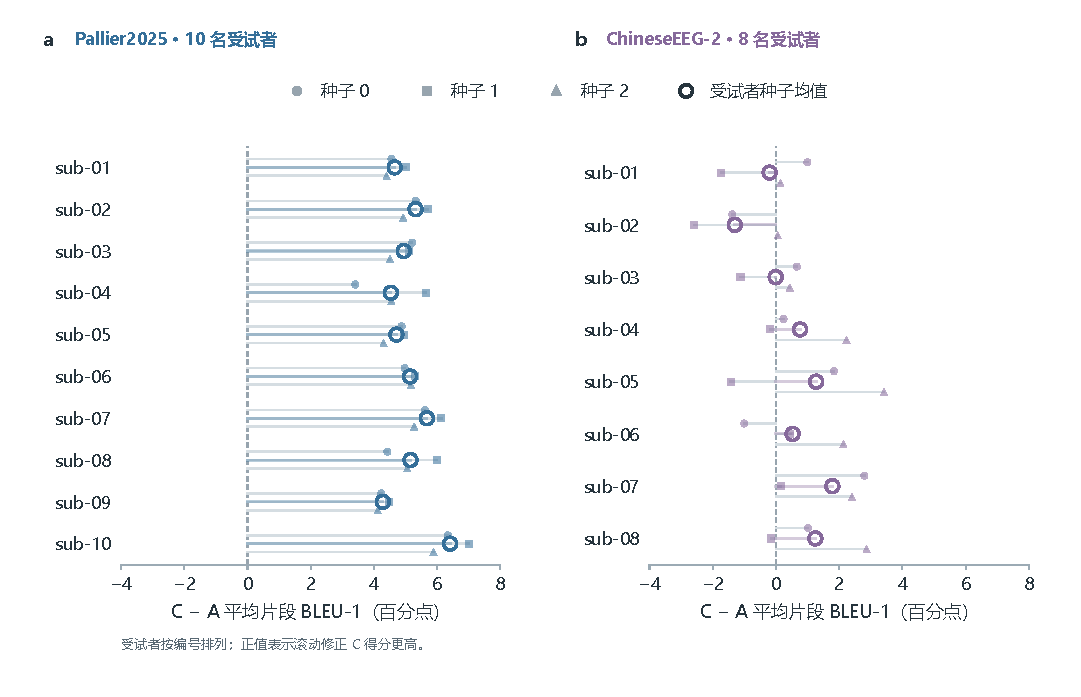
\includegraphics[width=\linewidth]{14_participant_gains.pdf}
    \caption{受试者层面 C 减 A 的平均片段 BLEU-1（百分点）。小符号为单个种子，空心圆为种子均值。ChineseEEG-2 的种子 $2$ 下 A 得分较低（$8.27\%$），种子 $1$ 的 C 减 A 为负。}
    \label{fig:sentence_participant_gains}
\end{figure}

\begin{table}[!htbp]
    \centering
    \papertablestyle
    \caption{全部测试词位的总输入等待（s）。等待从词起点计算，包含自身 $1\,\mathrm{s}$ 神经窗。}
    \label{tab:input_wait_complete}
    % Presentation only: simplify_appendix_tables_test_v2.py; verified frozen sources.
\begingroup
\papertablestyle
\begin{tabular}{@{}llrrrrr@{}}
\toprule
数据集 & 策略 & 词位数 & 均值 (s) & 中位 (s) & P90 (s) & \papertablehead{输入等待节省}{较 F (s)} \\
\midrule
Pallier2025 & A / K0 & 18450 & 1.000 & 1.000 & 1.000 & 2.311 \\
 & C / K2 & 18450 & 1.502 & 1.446 & 2.000 & 1.808 \\
 & F & 18450 & 3.311 & 2.342 & 6.670 & 0.000 \\
\addlinespace
ChineseEEG-2 & A / K0 & 8480 & 1.000 & 1.000 & 1.000 & 2.057 \\
 & C / K2 & 8480 & 1.542 & 1.480 & 2.120 & 1.514 \\
 & F & 8480 & 3.057 & 2.440 & 5.960 & 0.000 \\
\bottomrule
\end{tabular}
\endgroup

\end{table}

\begin{figure}[!htbp]
    \centering
    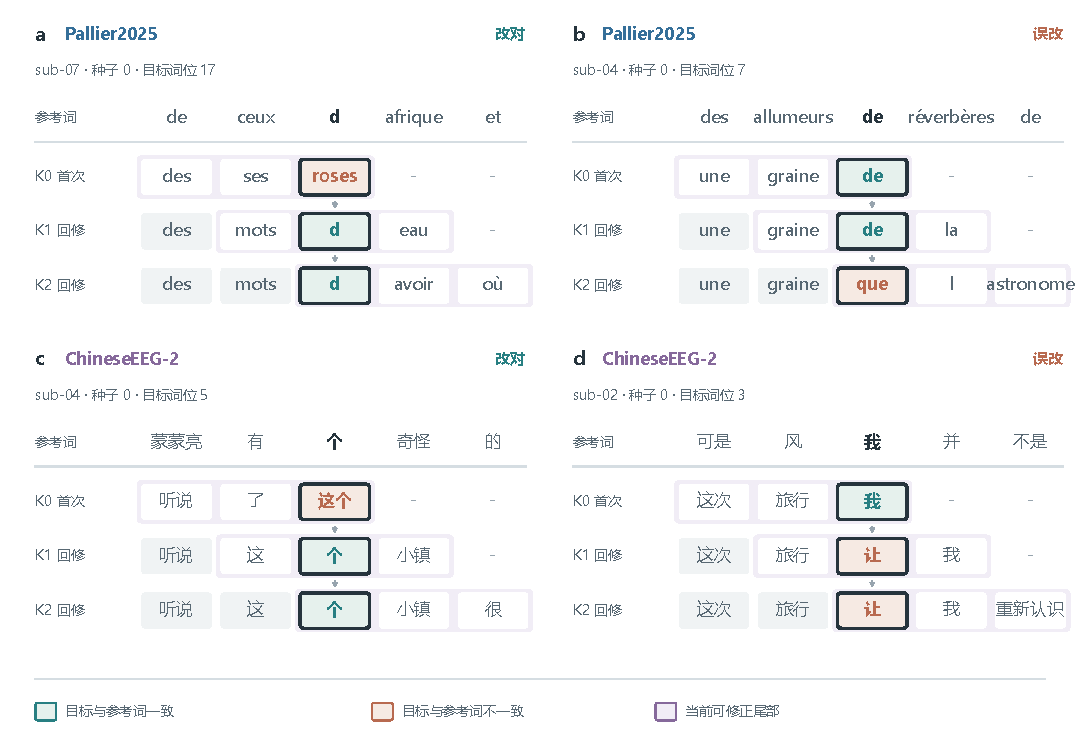
\includegraphics[width=\linewidth]{10_sentence_revision_examples.pdf}
    \caption{策略 C 的回修案例。三行依次为首次预测及两次回修；黑框标记目标词位，绿色和橙色分别表示与参考词一致和不一致。案例来自种子 $0$，各列对应固定词位。}
    \label{fig:sentence_examples_full}
\end{figure}
